%!TEX root = article.tex
\begin{figure}[t]
    \centering
    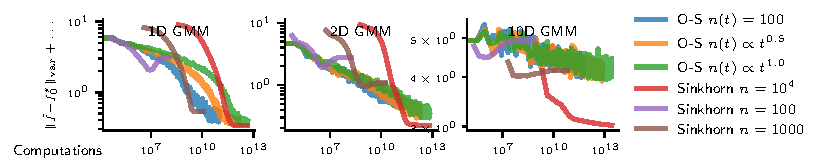
\includegraphics{online_0.01_False_test.pdf}
    \caption{Online Sinkhorn consistently estimate the true regularized OT potentials. Convergence here is measured in term of distance with potentials evaluated on a "test" grid of size $n=10^4$. Online-Sinkhorn can estimate potentials faster than sampling then scaling the cost matrix.}
    \label{fig:convergence}
\end{figure}

\begin{figure}[t]
    \centering
    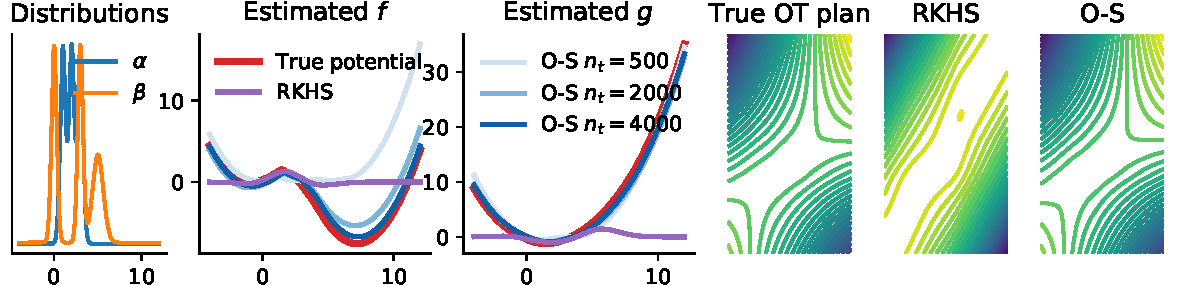
\includegraphics[width=\linewidth]{continuous.pdf}
    \caption{Online Sinhkorn finds the correct potentials over all space, unlike SGD over a RKHS parametrization of the potentials. The plan is therefore correctly estimated everywhere.}
    \label{fig:potentials}
\end{figure}

\section{Numerical experiments}\label{sec:exps}

% We have introduced and stated convergence results on the online Sinkhorn
% algorithm. These convergence results are non-quantitative and therefore
% require an experimental validation. Our experiments are three-fold: first, we
% show that online Sinkhorn correctly estimates the solutions of \eqref{eq:wass}
% and the Sinkhorn distance, overcoming the bias due to the fixed a priori
% sampling of the regular Sinkhorn algorithm. Then, we show how online Sinkhorn
% accelerates the Sinkhorn algorithm, by progressively estimating sketches of
% the dual potentials, in parallel to the computation of the distance matrix.
% Finally, we show how online Sinkhorn allows one to estimate accurately the
% geometry of the dual, significantly improving the result using SGD with RKHS
% expansions~\citep{2016-genevay-nips}.


The major purpose of online Sinkhorn (O-S) is to handle OT between continuous
distributions.  We first show that it is a valid alternative to applying Sinkhorn on a single realization of continuous distributions, using Gaussian mixtures. We illustrate how O-S accurately estimates the geometry of
the Kantorovich dual, significantly improving the result using SGD with RKHS
expansions~\citep{2016-genevay-nips}. Finally, we show that O-S
is an efficient warmup for accelerating Sinkhorn on real discrete problems.


% We first consider a discrete distribution $(\alpha, \beta)$, to be able to
% compute the reference distance $\Ww = \Ww(\alpha, \beta)$ and the optimal
% potentials $f^\star$, $g^\star$, using Sinkhorn algorithm. The goal here is not
% to perform better than the Sinkhorn algorithm in the long run. Indeed, the
% constraints of online Sinkhorn impose unnecessary slow-downs when dealing with
%  discrete distributions with small supports. Rather, our purpose is to illustrate the improved
% precision of online Sinkhorn for estimating true OT distances. We choose $\alpha$ and $\beta$ to be two
% discrete 1-D distributions, $\Xx=\RR$, sampled from the continuous densities
% displayed in
% \autoref{fig:potentials}. We set $\varepsilon = 10^{-2} \max_{x,y}
% C(x,y)$, where we use the squared Euclidean loss (regularized $\Ww_2$
% setting)---the distributions $\alpha$ and $\beta$ have bounded support. We use
% $\eta_t = \frac{1}{\sqrt{t}}$ for online Sinkhorn and a fixed batch-size $n$, in
% all experiments. We compare the performance of Sinkhorn, online Sinkhorn and
% random Sinkhorn, measuring $\Vert f - f^\star \Vert_{\text{var}} + \Vert g -
% g^\star \Vert_{\text{var}}$ and the absolute error $| \Ww_t - \Ww |$ versus the
% number of computations performed---the evaluation of $C(x_i, y_i)$ and the
% computation of each addition in the $C$-transform being considered as elementary
% computation units. We further report the performance of using out-of-loop
% averaging with $\gamma_t = \frac{1}{\sqrt{t}}$.

\subsection{Continuous potential estimation}\label{sec:continuous}

\paragraph{Data and quantitative evaluation.}\label{sec:online_exp}.We measure the performance of our algorithm in a
truly continuous setting, where $\alpha$ and $\beta$ are  parametric
distributions (Gaussian mixtures in 1D and 2D and 10D, with 3, 3 and 5 modes, so
that $C_{\max} \sim 1$), from which we draw samples. In the absence of reference
potentials $(f^\star, g^\star)$ (which cannot be computed without a method akin
to ours), we compute "test" potentials $(f^\star_0, g^\star_0)$ on realizations $\hat
\alpha_0$ and $\hat \beta_0$ of size $N=10000$, using Sinkhorn. We then compare
O-S to Sinkhorn runs of various size , trained on realizations $N=(100,1000,
10000)$ independent of the reference grid (to avoid reducing the problem to a
discrete problem between $\hat \alpha_0$ and $\hat \beta_0$). To measure
convergence, we compute $\delta_t = \Vert \hat f_t - f^\star_0 \Vert_{\var} +
\Vert \hat g_t - \tilde g_0 \Vert_{\var}$, evaluated on the grid defined by
$\hat \alpha_0$ and $\hat \beta_0$---an imperfect metric. We evaluate O-S with and without full-correction, with
different batch-size schedules (see \autoref{app:online_exp}), as well as the randomized Sinkhorn algorithm. Quantitative results are average over 5 runs. We report quantitative results for $\epsilon = 10^{-3}$ and non fully-corrective online Sinkhorn in the main text, and all other curves in supp. \autoref{fig:convergence_all}. In
supp. \autoref{fig:gaussian}, we also results for OT between Gaussians (arguably less useful), for which closed-form
potentials are known.

\paragraph{Comparison to SGD.}\label{sec:compare}
%
For qualitative illustration, on the 1D and 2D problem, we consider a competing
approach \citep{2016-genevay-nips}, in which $f_t(\cdot)$ is parametrized as
$\sum_{i=1}^{n_t} \alpha_t \kappa(\cdot, x_i)$ (and similarly for $g_t$), where
$\kappa$ is a reproducing kernel (typically a Gaussian). This differs
significantly from online Sinkhorn, where we express $e^{-f_t}$ as a Gaussian
mixture. The dual problem \eqref{eq:sinkhorn} is solved using SGD, with convergence guarantees on the dual energy.  As advocated
by the authors, we run a grid search over the bandwidth parameter~$\sigma$ of
the Gaussian kernel to select the best performing runs. 


\paragraph{Earlier potential convergence.} 
We report convergence curves in \autoref{fig:convergence}, comparing algorithms
at equal number of multiplications. For readability, we only report non
fully-corrective O-S results. Online Sinkhorn outperform or match Sinkhorn for $N=100$
and $N=1000$ on the three problems; it approximately matches the performance of
Sinkhorn on $N=10000$ new iterates on the 1D and 2D problems. On the two
low-dimensional problem, online Sinkhorn converges faster than Sinkhorn at the
beginning. Indeed, it starts potential computation early, while the Sinkhorn
algorithm must wait for the cost matrix to be filled;  this observation leads us
to study online Sinkhorn as a catalyser of Sinkhorn in the next paragraph. O-S
convergence is slower (but still happens) for the high dimensional problem.
Fully-corrective O-S performs better in this case (see supp. \autoref{fig:convergence_refit}). We note that
randomized O-S with batch-size $N$ performs on par with Sinkhorn of size $N$ (supp. \autoref{fig:convergence_randomized}).

\paragraph{Better-extrapolated potentials.} As illustrated in
\autoref{fig:potentials}, in 1D, online Sinkhorn refines the potentials $(\hat f_t, \hat g_t)_t$
until convergence toward $(f^\star, g^\star)$. Supp. \autoref{fig:potentials_2d} shows a visualisation for 2D GMM. As the parametrization~\eqref{eq:param} is 
adapted to the dual problem, the algorithm quickly identify the correct shape of
the optimal potentials---as predicted by \autoref{prop:convergence_true}. In
particular, O-S estimates potentials with much less errors than SGD in a RKHS in
areas where the mass of $\alpha$ and $\beta$ is low. This allow to consistently estimate the transport plan, which SGD cannot do. SGD did not converge
for $\epsilon < 10^{-1}$, while online Sinkhorn remains stable. Online
Sinkhorn does not require to set a bandwidth.


\begin{figure}[t]
    \begin{minipage}{.7\textwidth}
    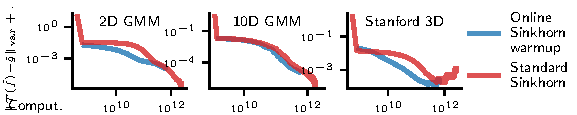
\includegraphics{online+full_0.001_err.pdf}
    \caption{Online Sinkhorn allows to warmup Sinkhorn during the evaluation of the cost matrix, and to speed discrete optimal transport.}
    \label{fig:warmup}
    \end{minipage}%
    \hfill
    \begin{minipage}{.25\textwidth}
        \small
        \begin{tabular}{lc}
            Dataset & Speed-up\\
            \toprule
            2D GMM & \\
            10D GMM & \\
            Stanford 3D & \\
            \bottomrule
        \end{tabular}
    \end{minipage}
\end{figure}


\subsection{Accelerating the first Sinkhorn iteration}\label{sec:accelerating}

The discrete Sinkhorn algorithm requires to compute the full cost matrix $\Cz
\eqdef (C(x_i,y_i))_{i,j}$  of size $N \times N$, prior to estimating the
potentials $\f_1 \in \RR^N$ and $\g_1 \in \RR^N$ by a first $C$-transform. In
contrast, online Sinkhorn can progressively compute this matrix while computing
first sketches of the potentials. The extra cost of estimating the initial potentials
without full-correction is simply $2 N^2$, i.e. similar to filling-up $\Cz$. We
therefore assess the performance of \textit{online Sinkhorn as Sinkhorn warmup}
in a discrete setting. Online Sinkhorn is run with batch-size $n$ during the
first iterations, until observing each sample of $[1,N]$, i.e. until the cost
matrix $\Cz$ is completely evaluated. From then, the
successor potentials are obtained using full Sinkhorn updates. We consider the
GMMs of \autoref{sec:continuous}, as well as a 3D dragon from Stanford 3D scans
\cite{turk1994zippered} and a sphere of size $N=12000$. We measure
convergence of the potentials in term with the error $\Vert
\Ctrans{\hat f_t}{\alpha} - \hat g_t \Vert_{\var} + \Vert \Ctrans{\hat
g_t}{\beta} - \hat f_t \Vert_{\var}$, evaluated on $\alpha$ and $\beta$; this error
goes to $0$. We use $n(t) = \frac{N}{100} (1+0.1t)^{1/2}$---results vary little on the exponent.


\paragraph{Results.} We report convergence curves for for $\varepsilon =
10^{-3}$ in \autoref{fig:warmup}. Convergence curves for different
$\varepsilon$ are reported in supp. \autoref{fig:warmup_full}. We report the speed-up
provided by online Sinkhorn in \autoref{table}. The proposed scheme provides an
improvement upon the standard Sinkhorn algorithm. After $N^2 d$ computations
(the cost of estimating the full matrix $C$), both the function value and
distance to optimum are lower using O-S: the full Sinkhorn updates then
relay the online updates, using a sound initialization of the potentials. The
\textit{O-S warmed-up} Sinkhorn algorithm then maintains an advantage over the
standard Sinkhorn algorithm over time. The speed gain increases
as $\varepsilon$ reduces and the OT problem becomes more complex. Sampling-without-replacement brings an additional speed-up.
